\problem
\begin{question}
    Consider $f(t,W_t)=e^{\alpha t+\beta W_t}$, $0\leq t\leq1$.

    (1)  Plot $f(t,W_t)$ with $(\alpha,\beta)=(0.5,0.5)$, $(\alpha,\beta)=(0.5,1)$, $(\alpha,\beta)=(1,0.5)$ and $(\alpha,\beta)=(1,1)$ in the graph.  For each process, plot two individual pathes.  Choose time steps $N=2000$.  Set your $y$--axis to $(0,5)$ and label each graph properly.

    (2)  Plot the means of $f(t,W_t)$ with $(\alpha,\beta)=(0.5,0.5)$, $(\alpha,\beta)=(0.5,1)$, $(\alpha,\beta)=(1,0.5)$ and $(\alpha,\beta)=(1,1)$ in the same graph.  Label and use different colors to distinguish your plots.  What are your observations?
\end{question}
\begin{subproblem}[(\arabic*)]
    \item See \cref{fig:GBM}.
    \item Since $E(f(t,W_t))=\exp((\alpha+\beta^2/2)t)$, we can
    plot it directly. As we can see in \cref{fig:GBM},
    $f(t,W_t)$ is oscillating around its expectation.
    Compare the two path with same $\alpha,\beta$, we can
    get an intuitive impression of the variation, and it
    it easy to find that
    greater $\beta$ means a greater variation.
    Similarly, compare different $\alpha$ with same $\beta$,
    we can conclude that $\alpha$ has a significant impact on 
    the trend of the curve.

    \begin{figure}[h]
        \centering
        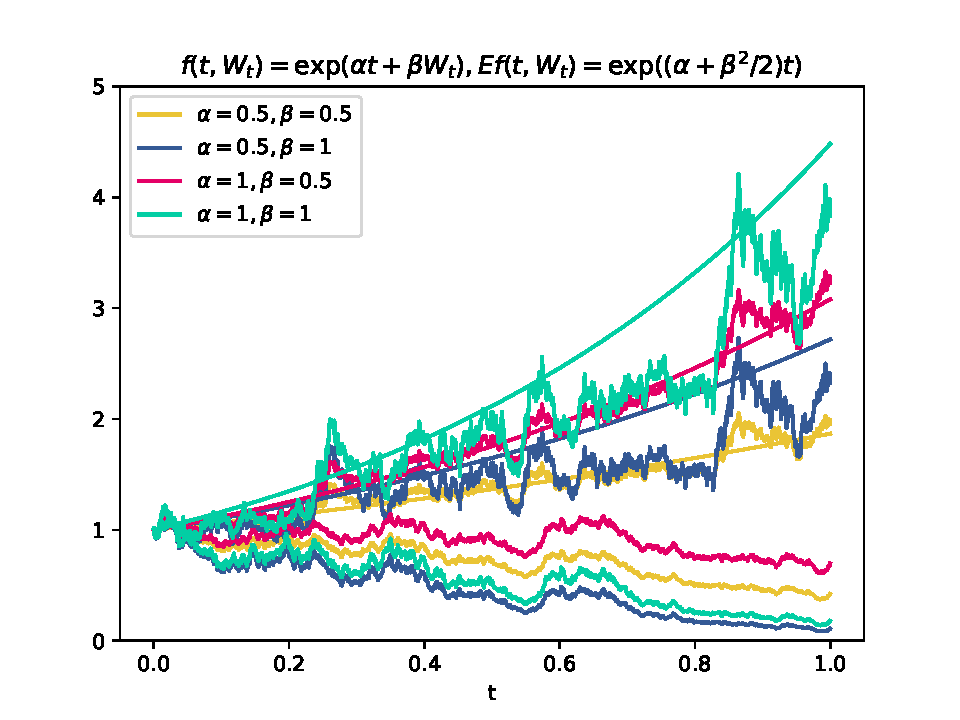
\includegraphics[width=\textwidth]{GBM}
        \caption{Graph of $f(t,W_t)$ and its expectation with different
        parameters. Here different curves correspond to different random events,
        since uniform random event comparison is not so interesting -- it
        is similar to the deterministic case.}
        \label{fig:GBM}
    \end{figure}
\end{subproblem}

\problem
\begin{question}
    Let $f=f(t,W_t)$, then we know that the It\^o and Stratonovich integrals are connected by the following identity
    \[\int_a^b f(t,W_t)\circ dW_t=\int_a^b f(t,W_t)dW_t+\frac{1}{2}\int_a^b \frac{\partial f(t,W_t)}{\partial W_t}\cdot dt.\]
    In particular, for $f(t,W_t)=W_t$ and $(a,b)=(0,1)$ we have that
    \[\int_0^1  W_t \circ dW_t=\int_0^1  W_t dW_t+\frac{1}{2}.\]

    Verify this identity by showing that the absolute difference between Strato and It\^o integrals converges to $\frac{1}{2}$ as the mesh step $N$ approaches to infinity.  To do this, denote
    \[E_N=|\text{Strato}_N-\text{It\^o}_N-\frac{1}{2}|\]
    and then make a table as $E_N$ against $N=2^k$, $k=2,4,6,8,10$ and $12$.  I would like to note that these integrals are stochastic processes themselves;
\end{question}
We can see from \cref{tab:diff} that the error tends to 0 as $N$ goes large.

\begin{margintable}
    \centering
    \begin{tabular}{cc}
        \toprule
        $k$ & error \\
        \midrule
        $2^{2}$ & $0.14513$\\
        $2^{4}$ & $0.26219$\\
        $2^{6}$ & $0.05478$\\
        $2^{8}$ & $0.04009$\\
        $2^{10}$ & $0.02272$\\
        \bottomrule
    \end{tabular}
    \caption{Difference Between It\^o and Stratonovich Integral}
    \label{tab:diff}
\end{margintable}

\problem
\begin{question}
    The Vasicek model is
    \[dr^V_t=\mu(b-r^V_t)dt+\sigma dW_t, r^V_0=r_0\]
    and the CIR model is
    \[dr^C_t=\mu(b-r^C_t)dt+\sigma \sqrt{r^C_t}dW_t, r^C_0=r_0.\]

    Numerically solve both equations and plot $r^V_t$ and $r^C_t$ in the same graphes over $t\in(0,10)$ for

    (1)  $r_0=10.1$, $b=10$, $\mu=1$ and $\sigma=1$;

    (2)  $r_0=10.1$, $b=10$, $\mu=0.1$ and $\sigma=1$;

    (3)  $r_0=10.1$, $b=10$, $\mu=0.01$ and $\sigma=1$;

    (4)  $r_0=10.1$, $b=10$, $\mu=0.01$ and $\sigma=0.01$;

    Then compare your results in (1)--(4) and describe your observations.
\end{question}
As we can see in \cref{fig:num}, in general,
the curves are oscillating around $b=10$, and bigger $\sigma$ means
more violent disturbation.
Compare the Vasicek and CIR model we see that, in general,
the curve of the former varies in a smaller range.

% TODO Description

\begin{figure}[h]
    \centering
    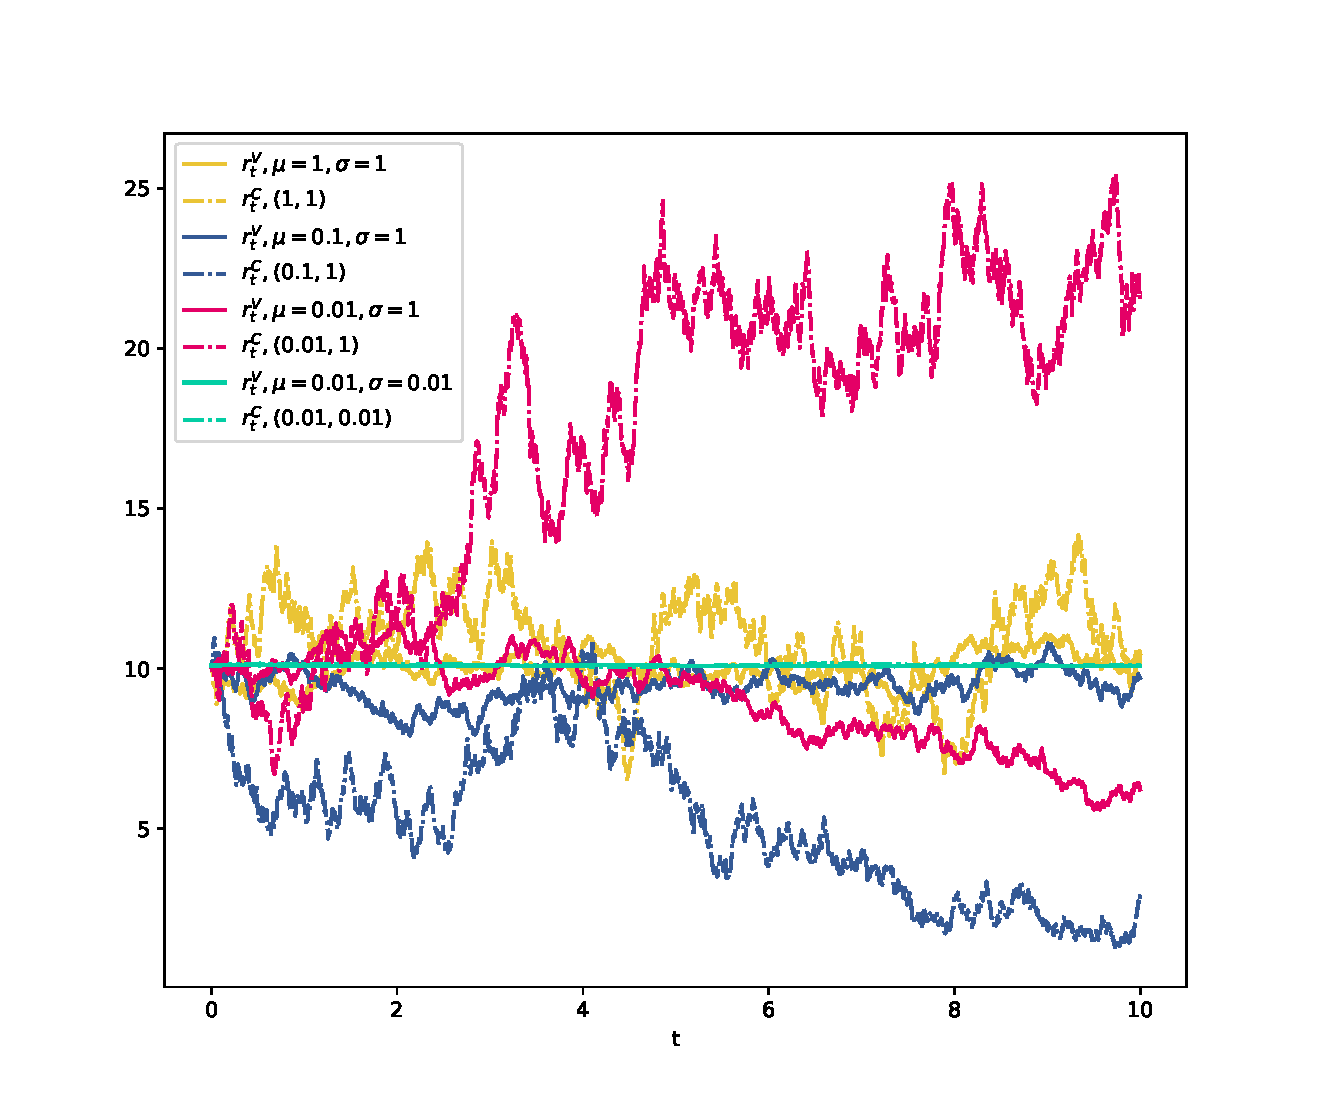
\includegraphics[width=\textwidth]{num}
    \caption{$r_t^V$ and $r_t^C$}
    \label{fig:num}
\end{figure}

\appendix
\section{Python Code}
\subsection{Code for Plotting $f(t,W_t)$}
\lstinputlisting[language=Python]{plot.py}
\subsection{Comparison of It\^o and Stratonovich}
\lstinputlisting[language=Python]{str-ito.py}
\subsection{Numerical Solution}
\lstinputlisting[language=Python]{numerical.py}